\par En su libro, \textit{Production Point} \cite{andersonProductionPointHow2023}, Anderson propone un framework para desarrollar juegos como solo dev. Para ello, separa el proceso en 2 etapas principales:
\begin{itemize}
  \item Pre-production: etapa exploratoria donde se experimentan con sistemas y mecánicas. Se busca la “diversión”, y esto se logra realizando prototipos e iterando sobre ellos. El objetivo es crear un vertical slice.
  \item Production: en esta etapa se crea contenido que apoya a las mecánicas obtenidas  en la preproducción. El objetivo es finalizar el juego.
\end{itemize}
\par Durante \textit{pre-production}(o pre-producción en español), el avance del proyecto sigue una curva exponencial. Esto es porque la integración de mecánicas se dificulta a medida que se añaden nuevas.  Un cambio pequeño puede tener un gran impacto en el juego. Por ejemplo, cambiar la altura del salto en un plataformero 2D puede representar que ciertas plataformas se vuelvan inaccesibles, o que la dificultad de un nivel cambie.
\par En cambio, el progreso durante \textit{production} (producción en español) es lineal. Esto se debe a que el foco es en crear contenido, no mecánicas nuevas. Por ejemplo, crear nuevos niveles debería en promedio tomar el mismo tiempo.
\begin{figure}[H]
  \centering
  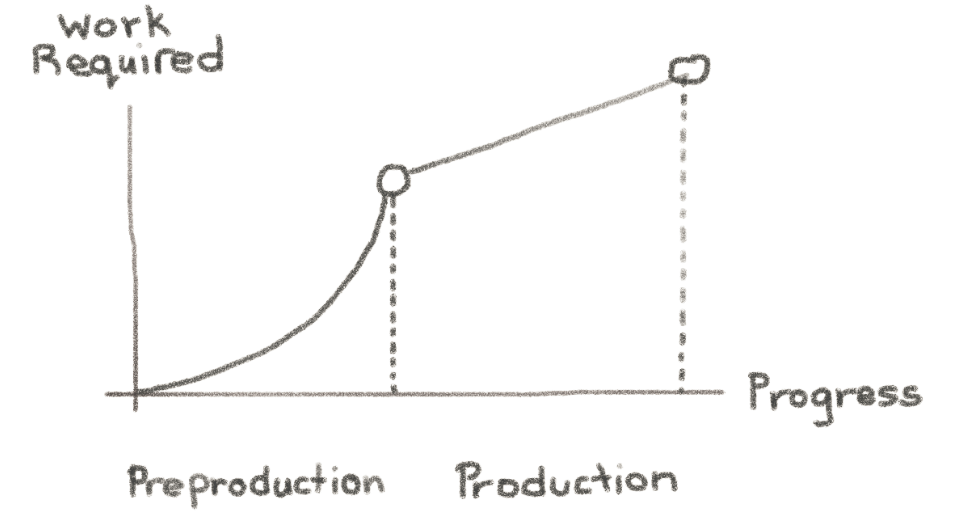
\includegraphics[scale=0.35]{image12.png}
  \caption{Gráfica que representa el progreso en las etapas de \textit{pre-production} y \textit{production}. Extraída de \cite{andersonProductionPointHow2023}.}
  \label{fig:x progreso de etapas Anderson}
\end{figure}
%
%
\subsection{Pre-production}
\par Como se mencionó anteriormente, durante esta etapa se trata de encontrar una mecánica (o varias de ellas) sobre las cuales construir un videojuego. Para ello, durante esta fase se pone un fuerte foco en realizar prototipos. La idea es validar ideas lo más rápido posible, descartando las que no funcionen e iterando sobre las que muestren potencial.
%
\subsubsection{Prototipado}
\par Para validar ideas, Anderson recomienda crear una gran cantidad de prototipos. Idealmente estos prototipos exploran mecánicas distintas, es decir que responden una pregunta de diseño única. Anderson recomienda 2 tipos de prototipado
\begin{itemize}
  \item Prototipos físicos: probar ideas con objetos de la vida real, como papel, juguetes, materiales como madera, etc. El aspecto positivo es que permiten explorar ideas rápidamente, ya que no requieren código o arte. Sin embargo, requieren un fuerte trabajo mental. Para juegos con daño o probabilidad, requiere realizar esos cálculos a mano.
  \item Prototipos digitales: como indica el nombre, son prototipos creados en una computadora. Anderson recomienda no preocuparse por la calidad del código o del arte. El objetivo es probar mecánicas, no crear un software pulido
\end{itemize}
\par Para Anderson, un buen espacio para prototipar son las game jams. En una game jam, los desarrolladores tienen un tiempo limitado para terminar un juego (3 días, 1 semana, etc). Además, suelen presentar al desarrollador con un tema sugerido. Por ejemplo, a finales de enero se realizó la Global Game Jam 2025, donde los participantes tuvieron 3 días para crear un videojuego que cumpliera con el tema “burbujas” \cite{globalgamejamGlobalGameJam2025}.
\bigbreak
\par Anderson también presenta la idea de un juego a la semana. Esta idea se basa en la experiencia de varios desarrolladores:
\begin{itemize}
  \item Bennet Foddy, profesor de game design en la Universidad de Nueva York, enseña una materia donde los alumnos deben crear un juego semanalmente y presentarlo al resto de la clase \cite{GameWeekTeaching}.
  \item “World of Goo” \cite{WorldGooSteam} fue creado en un programa llamado “Experimental Gameplay Project”, llevado a cabo en la Universidad Carnegie Mellon. Este proyecto también duraba una semana, y World of Goo fue uno de los prototipos que los creadores desarrollaron \cite{InterviewGrayGabler,Flashback2008Making}.
  \item Similarmente, “Downwell” \cite{DownwellSteam} fue uno de los prototipos semanales de su creador, Ojiro Fumoto \cite{crecenteHeresOnedev8month2015}. Este proceso fue inspirado por un artículo escrito por otro desarrollador, Ramil Ismail, que detalla los beneficios de realizar esta práctica \cite{GameWeekGetting}.
\end{itemize}
\par Durante esta fase, Anderson recomienda validar los prototipos mediante playtesting. El objetivo es obtener feedback abundante y preciso, que permita tomar decisiones informadas sobre una mecánica.
\par Idealmente, se tiene acceso a un grupo grande de personas que puedan probar el juego. Una gran cantidad de información facilita el proceso de entender el feedback recibido. Además, Anderson recomienda grabar las sesiones de playtesting, tanto el gameplay como la cara del tester. La utilidad de esto es poder observar las reacciones inmediatas de los jugadores.
%
\subsubsection{Vertical Slice}
El objetivo de la etapa de pre-producción es crear un vertical slice, es decir, una demo del juego que integra todas las partes de un videojuego. Esto incluye audio, arte, narrativa, interfaz de usuario y mecánicas. Anderson recomienda enfocarse en las siguientes áreas:
\begin{itemize}
  \item Arte y visuales: el aspecto visual de un videojuego es sumamente importante ya que es el primer punto de contacto que los jugadores tienen con un juego. Una buena manera de validar la dirección artística es creando \textit{mockups}\footnote{Mockup: Montaje de distintos elementos artísticos, como arte, sonido, colores, etc.} que incluyan arte, fuentes tipográficas y paletas de color que representen el aspecto visual que se busca. Luego, se puede pedir opiniones a otras personas sobre dicho \textit{mockup}.
  \item Sonido: Similar a las visuales, se pueden crear \textit{mockups} con música y sonidos. Anderson recomienda crear un sistema que permita cambiar los sonidos de objetos en el juego, de forma que se puedan probar rápidamente.
  \item Narrativa: Anderson recomienda utilizar los playtests grabados para validar la narrativa del juego. Con estos videos se puede observar si se está generando la emoción buscada.
  \item Interfaz de usuario: para esta área también se pueden utilizar \textit{mockups}, especialmente de otros juegos que estén en un género similar.
\end{itemize}
%
%
\subsection{Potential Point vs Production Point}
\par La tesis central de Anderson es encontrar el \textit{production point}, es decir, el punto donde pasar de pre-producción a producción. Finalizar la pre-producción no necesariamente significa que se puede avanzar a la siguiente etapa; el vertical slice puede haber tenido malos resultados, con mecánicas confusas y jugadores desinteresados. Anderson llama a este punto \textit{potential point}, e insiste que mover el proyecto a producción en ese momento puede llevar un proyecto al fracaso.
\par Anderson compara 2 prototipos; en el primero, Demonlocke, explica que avanzó a producción teniendo mecánicas sin finalizar, y poco interés por parte del público. En comparación, el segundo proyecto llamado Tic Tac Tanks, comenzó producción con las mecánicas ya definidas, y esta segunda etapa consistió en pulir el juego y añadir contenido.
\begin{figure}[H]
  \centering
  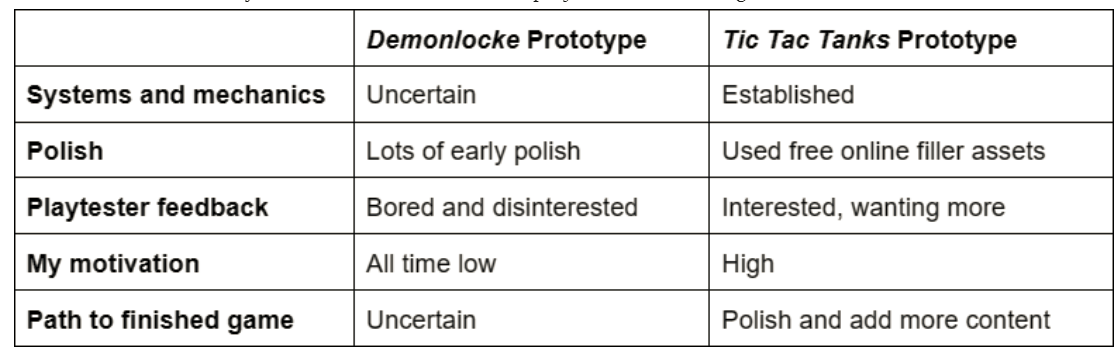
\includegraphics[scale=0.3]{image13.png}
  \caption{Comparación entre Demonlocke y Tic Tac Tanks. Extraída de \cite{andersonProductionPointHow2023}.}
  \label{fig:x Demonlocke vs tic tac tanks}
\end{figure}
\par Anderson propone una serie de preguntas que el proyecto debe contestar para saber en cuál de los puntos se encuentra:
\begin{itemize}
  \item ¿Funcionan todos los sistemas del juego?
  \item ¿Los playtesters disfrutan del juego?
  \item ¿Por cuánto tiempo juegan?
  \item ¿La gente se interesa inmediatamente por este juego a partir de las capturas de pantalla?
  \item ¿Se puede trazar un camino claro para finalizar el proyecto?
\end{itemize}
\par Si se contesta con “no” a alguna de estas preguntas, se recomienda tomar acciones que obtengan una respuesta afirmativa.
%
%
\subsubsection{Production}
\par El objetivo de esta etapa es construir un juego en base a las mecánicas obtenidas en pre-producción. Esto consiste en crear niveles, añadir una historia completa y pulir el arte y sonido. A diferencia de pre-producción, durante esta etapa es imperativo planificar el avance del proyecto y establecer fechas límite. Para ello, Anderson propone 3 acciones:
\begin{itemize}
  \item Establecer un tiempo de juego estimado: definir el largo del juego, generalmente en horas.
  \item Planificar cómo escalar el juego: para llegar a ese tiempo estimado, es importante encontrar formas de aumentar el contenido, lo cual depende del tipo de juego. Por ejemplo, un juego de plataformas tipo Mario Bros puede expandir el juego añadiendo niveles que pongan a prueba distintas habilidades del jugador.
  \item Utilizar herramientas como Kanban para visualizar el avance del proyecto.
\end{itemize}
%
%
\subsection{Alpha y Beta}
El objetivo de esta etapa es pulir el videojuego, de forma que esté preparado para salir al mercado. Algunas de las acciones recomendadas son:
\begin{itemize}
  \item Filtrar el contenido: realizado durante la fase de \textbf{alpha}, se elimina contenido del juego para crear un producto cohesivo. Un buen punto de partida es crear un formulario para quienes prueben el juego, con algunas preguntas como:
    \begin{itemize}
      \item ¿Cuál fue tu pieza de contenido favorita (nivel, personaje, enemigo, etc)?
      \item ¿Cuál fue la pieza de contenido que menos te gustó?
      \item ¿Cuál fue tu acción favorita (habilidad, ataque, etc)?
      \item ¿Cuál fue la acción que menos te gustó?
      \item ¿Si pudieras añadir algo al juego, qué sería?
    \end{itemize}
  \item Corregir bugs: como parte de la \textbf{beta}, se corrigen la mayor cantidad de bugs posible. Requiere tener un grupo grande de testers, que puedan probar el juego en distintas plataformas (Windows, Mac, Linux, Android, IOS, etc). Para mejorar la calidad de los reportes de errores, se recomienda crear un formulario que considere:
    \begin{itemize}
      \item Plataforma o sistema operativo
      \item Especificaciones de hardware
      \item Los pasos para recrear el bug
      \item De ser posible, screenshots o video
      \item Contacto (mail, discord, etc)
    \end{itemize}
  \item Implementar características de calidad de vida (QoL): cambios al juego que mejoran la experiencia de usuario.
  \item Implementar opciones de accesibilidad: esto consiste en opciones como modos de color para personas daltónicas, modificadores de dificultad, etc.
  \item Añadir localización: de ser posible, añadir nuevos idiomas al juego.
\end{itemize}
%
%
\subsection{Launch}
Parte del desarrollo incluye el lanzamiento del juego. Para ello, Anderson recomienda realizar el siguiente proceso:
\begin{enumerate}
  \item Establecer y anunciar la fecha de lanzamiento. Anderson recomienda realizar el anuncio un mes antes de publicar el juego, con el objetivo de formar interés por parte de los jugadores.
  \item Crear un press kit. Anderson define un press kit como “una colección de texto, imágenes, video del juego y trailers que puede enviarse a la prensa o creadores de contenido \footnote{Creador de contenido: Persona o equipo que crea material audiovisual y lo publica en redes sociales, como Youtube o Twitch.}” \cite{andersonProductionPointHow2023}.
  \item Crear un trailer de lanzamiento, indicando fecha de salida y lugar donde comprar el juego.
  \item Obtener lista de deseados. En plataformas como Steam [47] es imperativo que los potenciales compradores pongan el videojuego en su lista de deseados, ya que les avisará sobre el lanzamiento del mismo. Además, indica a los algoritmos de estas plataformas que hay interés por el juego y esto genera más chances de que sea recomendado a otras personas.
  \item Crear y testear una build \footnote{Build: archivos binarios del juego.} del juego. Muchas plataformas requieren cargar el juego con algunas semanas de anticipación. Este tiempo también es ideal para realizar una última ronda de tests.
  \item Esperar una semana antes de lanzar el juego. Utilizar esta semana para contactar a la prensa y creadores de contenido.
  \item Lanzar el juego.
\end{enumerate}
%
%
\subsection{Post Launch}
\par La última etapa del proceso consiste en revisar las críticas del juego y resolver los bugs que se encuentren. Anderson también menciona la posibilidad de expandir el juego con actualizaciones, sin embargo no entra en detalle de cómo realizar este proceso.
\bigbreak
\par En la figura 3.5 se puede observar el proceso completo:
\begin{figure}[H]
  \centering
  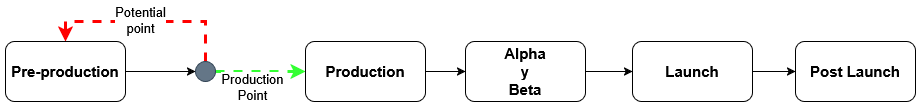
\includegraphics[scale=0.5]{image8.png}
  \caption{Proceso de desarrollo propuesto por Anderson. Creada por autor.}
  \label{fig:x proceso de desarrollo Anderson}
\end{figure}
